\chapter{Inertial Sensors and Their Errors}
\label{ch:imu}

\begin{objectives}
\begin{itemize}
  \item Understand how MEMS accelerometers and gyroscopes work, from Newton's law and the Coriolis effect.
  \item Understand specific force: what an accelerometer measures, and why it reads $+g$ at rest.
  \item State the IMU measurement model of the project, and the fuller error model of which it is a simplification.
  \item Know how IMUs are calibrated and how their noise parameters are measured and tuned.
  \item Convert between continuous-time noise densities, discrete per-sample noise, and datasheet units.
\end{itemize}
\end{objectives}

% ==============================================================================
\section{How a MEMS accelerometer works}

A MEMS (micro-electro-mechanical system) \term{accelerometer} is a tiny proof mass, a few micrograms of silicon, suspended on silicon springs inside a
case, with capacitive electrodes that measure its displacement relative to the case.

\begin{figure}[t]
\centering
\begin{tikzpicture}[scale=1.0]
  \draw[thick] (0,0) rectangle (6,2.4);
  \node[font=\small] at (0.55,2.1) {case};
  \draw[decorate, decoration={zigzag, amplitude=2.5mm, segment length=3mm}] (0,1.2) -- (2.2,1.2);
  \node[font=\footnotesize, above] at (1.1,1.45) {spring $k$};
  \draw[fill=primarylight, draw=primary, thick] (2.2,0.7) rectangle (3.4,1.7) node[pos=0.5] {$m$};
  \draw (3.4,1.2) -- (4.2,1.2);
  \draw (4.2,0.95) -- (4.2,1.45); \draw (4.0,0.85) -- (4.6,0.85) -- (4.6,1.55) -- (4.0,1.55);
  \draw (4.6,1.2) -- (6,1.2);
  \node[font=\footnotesize, above] at (4.4,1.6) {damper $c$};
  \draw[<->, conv] (2.2,0.45) -- (2.8,0.45) node[midway, below, font=\footnotesize] {$x$};
  \draw[dashed, conv] (2.2,0.35) -- (2.2,0.75);
  \draw[->, very thick, plotorange] (6.4,1.2) -- (7.6,1.2) node[right, font=\small] {$a_{\mathrm{case}}$};
  \draw[->, thick, black!60] (3.0,-0.2) -- (3.0,-0.9) node[right, font=\small] {$g$ (along the axis if tilted)};
\end{tikzpicture}
\caption{The spring-mass-damper model of an accelerometer. The displacement $x$ of the proof mass relative to the case is proportional, at low frequencies,
to the specific force along the sensitive axis.}
\label{fig:accel-model}
\end{figure}

\subsection{The spring-mass model}

Let the case have acceleration $a$ along the sensitive axis, let $g$ be the component of gravitational acceleration along that axis, and let $x$ be the
displacement of the mass relative to the case. The absolute acceleration of the mass is $a + \ddot x$, and the forces on it are the spring, the damper
and gravity (\cref{fig:accel-model}). Newton's law gives
\begin{equation}
  m(a + \ddot x) = -kx - c\dot x + mg
  \quad\Longrightarrow\quad
  \ddot x + 2\zeta\omega_n\dot x + \omega_n^2x = -(a - g),
  \label{eq:accel-dynamics}
\end{equation}
with natural frequency $\omega_n = \sqrt{k/m}$ and damping ratio $\zeta = c/(2\sqrt{km})$. At frequencies well below $\omega_n$ the derivative terms are negligible and
\begin{equation}
  x \approx -\frac{a - g}{\omega_n^2} .
\end{equation}
The deflection measures $a - g$, not $a$. Its frequency response, the ratio of $x$ to $-(a - g)/\omega_n^2$ for a sinusoidal input at angular frequency $\omega$, is
$1/(1 - (\omega/\omega_n)^2 + 2i\zeta\omega/\omega_n)$: flat below the resonance, peaked at it for small damping, falling off above it (\cref{fig:accel-bode}).
MEMS accelerometers resonate in the kHz range, and their electronics low-pass filter the output well below that, which also serves as the
anti-aliasing filter (\cref{ch:processes}).

\begin{figure}[t]
  \centering
  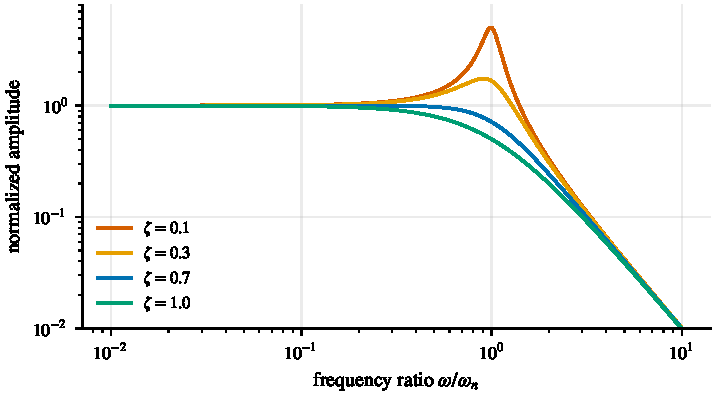
\includegraphics[width=0.84\textwidth]{fig_accel_bode.pdf}
  \caption{Frequency response of the spring-mass accelerometer model for several damping ratios. Below the natural frequency the response is flat: the
  deflection is proportional to specific force. A damping ratio near 0.7 gives the widest flat band without a resonant peak.}
  \label{fig:accel-bode}
\end{figure}

\subsection{Specific force}

\index{specific force}
The quantity measured is the \term{specific force}
\begin{equation}
  f = a - g,
\end{equation}
the non-gravitational force per unit mass acting on the sensor (the spring force divided by $m$). Gravity acts on the mass and the case equally
and cannot be felt directly: this is Einstein's equivalence principle. Two cases build intuition.
\begin{itemize}
  \item \textbf{At rest on a table}, $a = 0$, so $f = -g$. With $g_w = [0, 0, -9.81]\T$, the accelerometer reads $+9.81~\mathrm{m/s^2}$ \emph{upward}: it senses the table
        pushing it up.
  \item \textbf{In free fall}, $a = g$, so $f = 0$. A falling IMU reads zero, whatever its velocity.
\end{itemize}
To recover the kinematic acceleration from the measurement, the estimator rotates the specific force into the world frame and \emph{adds gravity back}:
$a_w = R_{wb}f_b + g_w$. A sign error here produces a vertical acceleration error of $2g \approx 20~\mathrm{m/s^2}$ and an obviously diverging altitude, which is
fortunately easy to recognize.

\paragraph{Noise.} Even a perfect mechanical sensor is noisy: the proof mass is jostled by the thermal motion of the surrounding gas, a
\emph{thermo-mechanical} noise whose acceleration density is about $\sqrt{4k_BT\omega_n/(mQ)}$ (with $k_B$ Boltzmann's constant, $T$ the temperature and $Q$ the
mechanical quality factor). Tiny masses are noisier, which is the basic trade-off of MEMS inertial sensing. Readout electronics add their own noise.

% ==============================================================================
\section{How a MEMS gyroscope works}

A MEMS \term{gyroscope} has no spinning wheel. It keeps a proof mass vibrating and detects the Coriolis force that rotation induces. Let the mass be
driven along the $x$-axis of the sensor at frequency $\omega_d$, so its velocity relative to the sensor is $v = A\omega_d\cos(\omega_dt)\,e_x$. If the sensor
rotates with angular velocity $\Omega$, then in the sensor frame the mass experiences the Coriolis acceleration $-2\Omega\times v$ (\cref{eq:coriolis}).
For a rotation about the $z$-axis this acceleration points along $y$:
\begin{equation}
  a_y = -2\,\Omega_z\,A\omega_d\cos(\omega_dt) .
\end{equation}
The resulting vibration along $y$ (the \emph{sense} mode) has an amplitude proportional to the rate $\Omega_z$ and oscillates at the drive frequency, so
the electronics recover $\Omega_z$ by demodulating the sense signal synchronously with the drive. The sensitive axis is perpendicular to both the drive and
the sense directions.

Real designs use two or four masses vibrating in anti-phase (a \emph{tuning fork}): their Coriolis forces are opposite and add in the differential
readout, while linear accelerations and vibrations push all masses the same way and cancel. Imperfect cancellation leaves a small sensitivity of the
gyro output to acceleration ($g$-sensitivity). Manufacturing asymmetries couple the drive into the sense mode (\emph{quadrature}), and their drift with
temperature is a major source of gyro bias.

% ==============================================================================
\section{The measurement model}

\subsection{The project's model}

\begin{convention}[IMU model, AGENTS.md C6]
\begin{equation}
  \omega_m = \omega_b + b_g + n_g, \qquad
  a_m = R_{wb}\T\big(a_w - g_w\big) + b_a + n_a, \qquad
  \dot b_g = n_{b_g}, \quad \dot b_a = n_{b_a},
  \label{eq:imu-model}
\end{equation}
with $\omega_m$, $a_m$ the gyroscope and accelerometer readings in the body frame, $\omega_b$ the true angular rate, $a_w$ the true acceleration of the body in the
world frame, $b_g$, $b_a$ the biases (body frame), and $n_g, n_a, n_{b_g}, n_{b_a}$ zero-mean white noises with densities $\sigma_g, \sigma_a, \sigma_{b_g}, \sigma_{b_a}$. The
noise vector is ordered $w = [n_a, n_g, n_{b_a}, n_{b_g}] \in \R^{12}$.
\end{convention}

The model has two kinds of error. \emph{White noise} ($n_g$, $n_a$) is independent from sample to sample and averages out. \emph{Bias} ($b_g$, $b_a$) is a slowly
varying offset that does not average out and is therefore estimated as part of the state (a shaping filter, \cref{ch:processes}). Its slow drift is
modeled as a random walk driven by $n_{b_g}$, $n_{b_a}$. Over the minutes of a EuRoC sequence the biases change little but measurably.

\subsection{A fuller error model}

High-accuracy inertial systems use a richer model, of which \eqref{eq:imu-model} is the special case $S = M = G = 0$:
\begin{equation}
  a_m = (I + S_a)M_a\,f_b + b_a + n_a, \qquad \omega_m = (I + S_g)M_g\,\omega_b + G_g\,f_b + b_g + n_g .
\end{equation}
Here $S$ is a diagonal matrix of \emph{scale-factor} errors (the output is $(1 + s)$ times the input), $M$ a near-identity matrix describing \emph{axis
misalignment and non-orthogonality} (the three sensing axes are neither exactly perpendicular nor exactly aligned with the body frame), and $G_g$ the
$g$-sensitivity of the gyroscope. Each of these parameters can be calibrated, estimated online as additional states, or ignored, at the cost of
some unmodeled error.

\begin{table}[t]
\centering\small
\begin{tabularx}{\textwidth}{@{}l X l@{}}
\toprule
\textbf{Error} & \textbf{Description} & \textbf{In the model?} \\
\midrule
White noise & sample-to-sample electronic and thermo-mechanical noise (angle/velocity random walk) & yes, $n_g$, $n_a$ \\
Turn-on bias & constant offset that differs at each power-up & yes, initial $b$ and $P_0$ \\
In-run bias drift & slow wandering of the offset & yes, random walk \\
Bias instability & flicker ($1/f$) noise floor of the bias & approximated by the random walk \\
Scale factor & output $= (1 + s)\times$ input & no \\
Axis misalignment & sensing axes not exactly orthogonal / aligned with the case & no \\
$g$-sensitivity & gyro output depends on acceleration & no \\
Temperature effects & bias and scale factor change with temperature & no (absorbed by bias walk) \\
Quantization & finite resolution of the ADC & no (below white noise) \\
Saturation, vibration & clipping on impacts; aliasing of high-frequency vibration & no \\
Earth rotation & gyros sense $7.3\times10^{-5}$~rad/s & no (\cref{ch:rotations}) \\
\bottomrule
\end{tabularx}
\caption{IMU error sources and how the project's model treats them.}
\label{tab:imu-errors}
\end{table}

\Cref{tab:imu-errors} lists the main error sources. Unmodeled errors do not disappear: they appear as apparent extra noise or apparent bias drift. A filter
that ignores them must compensate with larger noise parameters than the white-noise floor alone would suggest, which is why tuning is needed even with a
well-calibrated sensor. The size of the effect is easy to estimate: a scale-factor error of $10^{-3}$ on a gyro turning at 1~rad/s is an apparent bias of
$10^{-3}$~rad/s, as large as a poor bias and much larger than the EuRoC gyro's noise.

% ==============================================================================
\section{Calibration}

\paragraph{Gyroscope bias.} At rest, the gyroscope should read zero (or the Earth rate). Averaging a few seconds of data gives the bias, with a standard
deviation of $\sigma_g/\sqrt T$ after $T$ seconds (\cref{ch:processes}): for EuRoC, $10^{-4}$~rad/s after 3~s.

\paragraph{Accelerometer bias and scale: the six-position test.} Place the IMU with each axis pointing straight up and then straight down. For an axis with
bias $b$ and scale factor $1 + s$, the two readings are $(1 + s)g + b$ and $-(1 + s)g + b$, so
\begin{equation}
  b = \frac{a_{\mathrm{up}} + a_{\mathrm{down}}}{2}, \qquad 1 + s = \frac{a_{\mathrm{up}} - a_{\mathrm{down}}}{2g} .
\end{equation}
Using more orientations and a least-squares fit (\cref{ch:estimation}) also yields the misalignments.

\paragraph{Gyroscope scale and misalignment.} These require known rotations, from a rate table, or from a known sequence of orientations measured by an
accelerometer.

\paragraph{Camera--IMU calibration.} The extrinsic transform $T_{bc}$, the time offset between the sensors, and optionally the IMU's own scale and misalignment
are estimated jointly by moving the rig in front of a calibration target. The Kalibr toolbox~\cite{furgale2013kalibr}, which produced EuRoC's calibration,
represents the trajectory as a continuous-time B-spline and solves one large nonlinear least-squares problem (\cref{ch:nlls}) combining camera
reprojection errors and IMU residuals.

\paragraph{Temperature.} Biases and scale factors depend on temperature. Industrial IMUs are calibrated at several temperatures and compensated with an
on-board temperature sensor; consumer IMUs often are not, and a filter must track the resulting drift as bias random walk.

% ==============================================================================
\section{Noise parameters and their units}

The noise densities are continuous-time quantities (\cref{sec:ct-noise}). For EuRoC's ADIS16448, the \code{imu0/sensor.yaml} file gives the values in
\cref{tab:euroc-imu}.

\begin{table}[h]
\centering\small
\begin{tabular}{@{}l l l l@{}}
\toprule
YAML key & Symbol & Value & Units \\
\midrule
\code{gyroscope\_noise\_density} & $\sigma_g$ & $1.6968\times10^{-4}$ & $\mathrm{rad/s/\sqrt{Hz}}$ \\
\code{accelerometer\_noise\_density} & $\sigma_a$ & $2.0\times10^{-3}$ & $\mathrm{m/s^2/\sqrt{Hz}}$ \\
\code{gyroscope\_random\_walk} & $\sigma_{b_g}$ & $1.9393\times10^{-5}$ & $\mathrm{rad/s^2/\sqrt{Hz}}$ \\
\code{accelerometer\_random\_walk} & $\sigma_{b_a}$ & $3.0\times10^{-3}$ & $\mathrm{m/s^3/\sqrt{Hz}}$ \\
\code{rate\_hz} & $1/\Dt$ & 200 & Hz \\
\bottomrule
\end{tabular}
\caption{EuRoC IMU noise parameters (\code{imu0/sensor.yaml}). Verify against your copy of the dataset.}
\label{tab:euroc-imu}
\end{table}

The units follow from the definitions. A gyro rate in rad/s with a white noise density has units $\mathrm{rad/s}\cdot\sqrt{\mathrm{s}} = \mathrm{rad/s/\sqrt{Hz}}$. A gyro
bias random walk is the integral of white noise with units of $\mathrm{rad/s^2}$, so its density is in $\mathrm{rad/s^2/\sqrt{Hz}}$, and after $t$ seconds the
bias has standard deviation $\sigma_{b_g}\sqrt t$ in rad/s.

\paragraph{Discrete equivalents.} At sample period $\Dt$ (\cref{eq:discrete-noise}):
\begin{equation}
  \sigma_{g,d} = \frac{\sigma_g}{\sqrt\Dt}, \qquad \sigma_{a,d} = \frac{\sigma_a}{\sqrt\Dt}, \qquad
  \sigma_{b_g,d} = \sigma_{b_g}\sqrt\Dt, \qquad \sigma_{b_a,d} = \sigma_{b_a}\sqrt\Dt .
\end{equation}
For EuRoC: $\sigma_{g,d} = 2.4\times10^{-3}$~rad/s per sample, $\sigma_{a,d} = 2.8\times10^{-2}~\mathrm{m/s^2}$ per sample, and the gyro bias diffuses by
$1.4\times10^{-6}$~rad/s per sample. In the filter you never need these directly, because $Q_d = G_cQ_cG_c\T\Dt$ uses the densities, but they are what a synthetic
data generator must add to each sample.

\paragraph{Datasheet units.} Manufacturers often quote angle random walk (ARW) in $^\circ/\sqrt{\mathrm{h}}$ and velocity random walk (VRW) in $\mathrm{m/s/\sqrt{h}}$.
Since $1\ ^\circ/\sqrt{\mathrm{h}} = \frac{\pi/180}{60}~\mathrm{rad/\sqrt{s}} = 2.909\times10^{-4}~\mathrm{rad/s/\sqrt{Hz}}$, EuRoC's $\sigma_g$ is an ARW of $0.58\ ^\circ/\sqrt{\mathrm{h}}$,
and its $\sigma_a$ is a VRW of $0.12~\mathrm{m/s/\sqrt{h}}$. Bias instability is quoted in $^\circ/\mathrm{h}$ and is \emph{not} the same thing as the random walk
density.

\paragraph{Measuring them.} The densities are measured from a long static recording with the Allan variance (\cref{sec:allan,fig:allan}): white noise is read
off the slope $-\tfrac12$ at $\tau = 1$~s, and the bias random walk off the slope $+\tfrac12$ at $\tau = 3$~s.

% ==============================================================================
\section{Tuning in practice}

The densities from an Allan analysis describe a stationary sensor in a quiet lab. On a flying vehicle, vibration, temperature changes, scale-factor and
misalignment errors, timing jitter and integration error all add to the effective noise. Common practice is to start from the Allan values (or the
dataset's values) and inflate them by a modest factor until the filter is consistent, as judged by the statistical tests of \cref{ch:consistency}. Two
rules keep tuning honest.
\begin{enumerate}
  \item \textbf{Change physically meaningful parameters only}, and keep them within a plausible range of their measured values.
  \item \textbf{Judge on consistency statistics} (NEES on synthetic data, NIS and $3\sigma$ coverage on real data), not on trajectory error alone. Tuning for
        the lowest trajectory error on the test sequence is overfitting.
\end{enumerate}

\begin{pitfall}[mixing up the two discretizations]
The white-noise variance per sample is $\sigma^2/\Dt$ (larger at higher rate), while the random-walk variance per step is $\sigma_b^2\Dt$ (smaller at higher rate).
Swapping them is a common bug in synthetic data generators, and it produces noise that is wrong by a factor of $1/\Dt^2 = 40\,000$ at 200~Hz.
\end{pitfall}

\section{The EuRoC IMU stream}

EuRoC's \code{imu0/data.csv} contains one row per sample: \code{timestamp [ns], w\_x, w\_y, w\_z [rad/s], a\_x, a\_y, a\_z [m/s\textsuperscript{2}]}, i.e.\ $\omega_m$
and $a_m$ in $B$ (AGENTS.md C7). Samples arrive at nominally 200~Hz, hardware-synchronized with the cameras. The filter must nevertheless take $\Dt$ from
consecutive timestamps (AGENTS.md C5): real data has jitter and occasional gaps, which Milestone 3 logs. The ground-truth file starts later than the IMU
file, so the filter is initialized at the first ground-truth sample at or after the stream start.

\begin{projectlink}[Milestones 3 and 4]
M3 parses \code{sensor.yaml} into exactly the parameters of \cref{tab:euroc-imu} and builds the event stream. M4's synthetic trajectory generator produces
noise-free IMU data from \eqref{eq:imu-model}; adding noise with the discrete equivalents above turns it into the Monte Carlo generator of M5.
\end{projectlink}

\begin{takeaways}
\begin{itemize}
  \item An accelerometer is a spring-mass system whose deflection, below resonance, is proportional to specific force $f = a - g$: it reads $+g$ upward at rest
        and zero in free fall.
  \item A MEMS gyroscope measures the Coriolis force on a vibrating mass.
  \item $\omega_m = \omega_b + b_g + n_g$ and $a_m = R_{wb}\T(a_w - g_w) + b_a + n_a$, with random-walk biases; scale factors and misalignments are neglected.
  \item Biases and scale factors can be calibrated with static multi-position tests; camera--IMU extrinsics with a target and a continuous-time solver.
  \item Noise densities have units of $[u]/\sqrt{\mathrm{Hz}}$; per-sample white noise is $\sigma/\sqrt\Dt$, per-step bias diffusion is $\sigma_b\sqrt\Dt$.
  \item Unmodeled errors force noise inflation; tune on consistency, not on accuracy.
\end{itemize}
\end{takeaways}

\begin{exercises}
  \item An IMU lies on a table tilted by $10^\circ$ about its $x$-axis. Compute the ideal accelerometer reading. Which component reveals the tilt, and with what sign?
  \item A MEMS accelerometer has a resonance at 5~kHz. How large is its static deflection per $\mathrm{m/s^2}$? Compare with the size of a silicon atom
        ($\approx 0.2$~nm) and comment.
  \item Derive the gyroscope's Coriolis acceleration from \eqref{eq:coriolis}, and explain why a tuning-fork design rejects linear acceleration.
  \item A six-position test gives $a_{\mathrm{up}} = 9.83$ and $a_{\mathrm{down}} = -9.79~\mathrm{m/s^2}$ on one axis. Compute the bias and scale factor.
  \item A gyroscope datasheet gives ARW $= 0.2\ ^\circ/\sqrt{\mathrm{h}}$. Convert it to $\mathrm{rad/s/\sqrt{Hz}}$ and to the per-sample standard deviation at 400~Hz.
  \item A scale-factor error of $s = 10^{-3}$ affects a gyro on a vehicle spinning at 1~rad/s. What equivalent bias does it produce? Why can't a constant-bias model
        absorb it during maneuvers?
\end{exercises}
